\chapter{Processo}

Neste capítulo, pretende-se abordar o processo escolhido, explicando as suas \textit{lines} e descrevendo cada atividade dentro desse fluxo. Dessa forma, o documento está estruturado em 4 tópicos, para cada uma das respectivas \textit{lines}.

\section{Line 1 - Analisar Problema}

\subsection{Identificar Envolvidos}
\subsubsection{Descrição}
  Essa atividade tem como foco descrever todos os interessados e afetados pela aplicação a ser desenvolvida. Isso é, a empresa júnior Engrena. A equipe de desenvolvimento e até mesmo os monitores da disciplina, bem como a professora, entram nesse contexto.
  Além disso, pretende-se aprofundar um pouco mais essa visão, ao descrever não somente os interessados e afetados pelo sistema, como também os seus usuários diretos.

\subsubsection{Relato}
  Essa atividade foi realizada com o auxílio de entrevistas, principalmente. Encontros foram marcados todas as terças-feiras às 12h com o cliente. Foi a atividade introdutória de todo o processo de Engenharia de Requisitos desenvolvida pela equipe.

\subsubsection{Resultado}
  Como resultado dessa atividade, houve um documento especificando os envolvidos do projeto. É importante ressaltar que esse documento evoluiu e se tornou uma parte do documento de visão, presente nos apêndices do documento. Os envolvidos, basicamente, são:

\textbf{Envolvidos:}
  \begin{itemize}
  \item Equipe de Desenvolvimento
  \item Gustavo Sabino, monitor da disciplina
  \item Professora Elaine Venson
  \item Romenigue Igor Melo Araujo Fernandes, representante da empresa
  \item Engrena, empresa júnior da Faculdade do Gama
  \end{itemize}

\textbf{Usuários:}
\begin{itemize}
\item Diretores e gestores da Engrena
\item Funcionários da Engrena
\end{itemize}

\subsection{Entender o Contexto da Empresa}
\subsubsection{Descrição}
  Essa atividade objetiva tornar clara a situação atual da empresa, descrevendo o problema a ser solucionado pela equipe. Ou seja, é a parte do processo em que é discutido explicitamente o que é esperado da solução a ser desenvolvida.

\subsubsection{Relato}
  Essa atividade também foi realizada com o auxílio de entrevistas, que consiste em uma técnica de elicitação muito eficaz em inícios de projetos. Durante essa atividade, foi criada uma intimidade maior com o cliente e a equipe, tornando o clima mais informal e propiciando o avanço de uma simples entrevista para uma conversa mais fluida e completa sobre o contexto da empresa, evitando que algum detalhe não fosse capturado.

\subsubsection{Resultado}
  Como saída dessa atividade, foi realizado um documento especificando o contexto da empresa que foi utilizado inclusive no primeiro relatório da disciplina.

\subsection{Entender Regras da Empresa}
\subsubsection{Descrição}
  As regras da empresa é uma atividade complementar a anterior no sentido de que aprofunda o contexto de uso da aplicação a ser desenvolvida. Isso porque, dependendendo das regras que regulamentam a empresa júnior, certas características seriam alteradas no decorrer do projeto.

\subsubsection{Relato}
  Essa atividade foi desenvolvida de forma mais interna, de forma a não envolver o cliente de forma tão intensa. A saída da atividade anterior foi utilizada como insumo para essa, objetivando verificar se tudo que havia para ser capturado sobre a empresa foi de fato capturado. As interações com o cliente foram meramente de consulta, em caso de dúvidas.

  \subsubsection{Resultado}
    Como saída dessa atividade, foi realizado um documento especificando as regras da empresa, isso é, a forma como a mesma opera. São elas:

    \begin{description}
    \item [Rotatividade de funcionários] Dentro do contexto da empresa júnior Engrena, existe a política de rotatividade adotado, se espelhando em várias outras empresas que obtiveram sucesso não apenas na satisfação do empregado, retirando o sentimento de monotonia e identificando quais características emergem do funcionário, podendo assim encaminhar o mesmo para uma área mais adequada.

    \item [Desempenho dos funcionários] A Engrena possui uma grande dificuldade em identificar e exibir para os diretores como um funcionário está desempenhando o seu papel dentro da empresa, atualmente processando-se através de planilhas no Excel®, desta forma exibindo apenas resultados binários da execução de tarefas.

    \item [Identificação de prováveis diretores] Dentro da política da Engrena, existe uma filosofia de promoção de funcionários através de suas habilidades e desempenho. Com o atual cenário de muitos diretores terem se formado, surgiu uma grande demanda para os cargos de diretores, porém com a vigente estrutura de reconhecimento do desempenho, esta filosofia está quase que impossibilitada.

    \item [Entrada de pessoas sem experiência técnica] Por se tratar de uma empresa júnior, o ingresso de pessoas na Engrena é feito sem a necessidade obrigatória de muita experiência técnica. Isso é, o único requisito para se tornar um funcionário da empresa é estar disposto a aprender novas coisas frequentemente.

    \end{description}


\subsection{Desenvolver Visão}
\subsubsection{Descrição}
  Atividade que tem como objetivo desenvolver o Documento de Visão, que estabelece um marco entre todos os envolvidos do projeto sobre o que será desenvolvido. Ou seja, o documento é um consenso entre as partes do projeto acerca dos envolvidos, usuários, problemas, necessidades e características.

\subsubsection{Relato}
  O desenvolvimento do Documento de Visão se deu sem maiores complicações, devido a qualidade da interação entre a equipe e o cliente nas atividades anteriores. Utilizou como insumo todos os conhecimentos e artefatos gerados nas atividades anteriores.

\subsubsection{Resultado}
  Essa atividade teve como saída o Documento de Visão, presente nos apêndices deste documento. Ao fim dessa atividade, ocorreu a validação com o cliente do documento gerado.

\section{Line 2 - Compreender as Necessidades dos Envolvidos}
\subsection{Identificar características do produto}
\subsubsection{Descrição}
Essa atividade serviu como revisão para o Documento de Visão. Isso é, as características do produto presentes no documento citado deveriam ser revistas e validadas novamente para prevenção contra erros futuros advindos da má identificação das mesmas.

\subsubsection{Relato}
Foi desenvolvida com o cliente através da revisão ao que já fora produzido em atividades anteriores. As técnicas de entrevistas foram novamente utilizadas para reafirmar os valores das informações previamente obtidas.

\subsubsection{Resultado}
Complemento no documento de visão acerca dos problemas e necessidades do cliente das características do produto. São elas:

\textbf{Problemas}
\begin{itemize}
\item PB1: Gerenciar os membros e as atividades dos mesmos.
\end{itemize}

\textbf{Necessidades}
\begin{itemize}
\item NE1.1: Verificar desempenho de áreas e usuários individuais dentro da empresa. Também consultar tal informação relativo ao tempo.
\item NE1.2: Criar tarefas em um ambiente virtual compartilhado e assinalar funcionários para sua execução, com atributos.
\end{itemize}

\textbf{Características}
\begin{itemize}
\item CA 1.1.1: Agregar informações.
\item CA 1.1.2: Mostrar desempenho de membros graficamente.
\item CA 1.2.1: Criar tarefas em um ambiente virtual.
\item CA 1.2.2: Verificar tarefas completadas.
\item CA 1.2.3: Criar áreas para alocação de membros.
\end{itemize}

\subsection{Levantar RF}
\subsubsection{Descrição}
Desenvolvida as características do produto, o próximo passo foi convertê-las em requisitos funcionais, isso é, descrição de funcionalidades que deverão ser providas pelo sistema.

\subsubsection{Relato}
Atividade mais marcante do processo devido à utilização das técnicas de cenário e quadro branco, introduzida pelo professor Fernando Wanderley nas aulas da disciplina. Essas técnicas complementaram-se de forma surpreendente na reunião com o cliente destinada a essa atividade e à atividade de "Levantar RNF" (isso é, as duas atividades foram desenvolvidas com as mesmas técnicas na mesma reunião). A equipe fornecia um cenário e enquanto o mesmo era discutido, as partes do projeto utilizavam o quadro branco para aprofundar as informações obtidas.

\subsubsection{Resultado}
O resultado dessa atividade são os requisitos funcionais não documentados. Ou seja, a saída dessa atividade serve de insumo para a elaboração do documento "Especificação de Requisitos de \textit{Software}".

\subsection{Identificar Casos de Uso}
\subsubsection{Descrição}
  Capturados os requisitos funcionais, essa atividade serve como introdução aos casos de uso, para que os mesmos contemplem os requisitos previamente coletados.

\subsubsection{Relato}
  Com as informações obtidas do levantamento de requisitos funcionais, foi possível elaborar o artefato de saída dessa atividade: Diagrama de Casos de Uso. Nele, foram especificados de forma simples a fronteira do sistema, bem como os atores e as interações com os casos de uso.

  \clearpage{}
  
  \subsubsection{Resultado}
  A saída dessa atividade é a geração do Diagrama de Casos de Uso:

  \begin{figure}[!ht]
  	\centering
  	\label{figura_Diagrama-de-Caso-de-Uso}
  		\includegraphics[keepaspectratio=true,scale=0.6]{figuras/Diagrama-de-Caso-de-Uso.eps}
  	\caption{Diagrama de Caso de Uso}
  \end{figure}


\subsubsection{Modelar Casos de Uso}
\subsubsection{Descrição}
  Essa tarefa consiste em especificar os casos de uso descritos no Diagrama de Casos de Uso, introduzindo elementos que servem para aprofundar os mesmos.

\subsubsection{Relato}
  Foram produzidos as especificações dos casos de uso identificados, introduzindo pré-condições, pós-condições, fluxos e regras de negócio.

\subsubsection{Resultado}
  Foi produzido o documento de "Especificação de Casos de Uso". Esse documento, complementado com o diagrama previamente elaborado, constitui o Modelo de Caso de Uso que nomeia a atividade. O documento citado está nos apêndices deste documento. Os casos de uso são:
  \begin{itemize}
  \item Manter membro;
  \item Manter área;
  \item Manter tarefas;
  \item Atribuir tarefas à funcionário;
  \item Gerar gráficos de produtividade de membros e área;
  \item Assinalar \textit{status} das tarefas
  \end{itemize}

\subsection{Levantar RNF}
\subsubsection{Descrição}
Atividade que serve para levantar os requisitos não funcionais da aplicação, isso é, o comportamento esperado para a mesma que não inclui funcionalidades.

\subsubsection{Relato}
Atividade que foi produzida em conjunto com "Levantar RF", não havendo necessidade de relatar novamente.

\subsubsection{Resultado}
O resultado dessa atividade são os requisitos não funcionais não documentados. Ou seja, a saída dessa atividade serve de insumo para a elaboração do documento "Especificação Suplementar".

\subsection{Elaborar Especificação Suplementar}
\subsubsection{Descrição}
Essa atividade serve para documentar os requisitos não funcionais capturados na atividade de "Levantar RNF", de forma a prover fácil acesso aos mesmos.

\subsubsection{Relato}
Foi uma atividade simples de documentação, sem maiores complicações.

\subsubsection{Resultado}
A saída dessa atividade é o documento de "Especificação Suplementar", presente nos apêndices deste documento.

\subsection{Validar com o Cliente}
\subsubsection{Descrição}
Objetiva validar todos os artefatos gerados nessa \textit{line}.

\subsubsection{Relato}
Foi uma atividade crucial para o projeto, pois se os artefatos gerados fossem recusados pelo cliente, a \textit{line} inteira teria que ser refeita.

\section{Line 3 - Planejar Iteração}

\subsection{Refinar Cronograma}
Nessa atividade, o cronograma do projeto foi atualizado para que a equipe pudesse verificar em que estado se encontrava dentro do processo em relação a disciplina. Foi realizada com o auxílio da ferramenta de calendário Gantter.

\subsection{Priorizar Casos de Uso}
Essa atividade tem como objetivo analisar quais casos de uso serão priorizados para a implementação dentro da disciplina. Foi realizada durante o segundo Ponto de Controle da disciplina, com o auxílio dos monitores da mesma.

\subsection{Produzir Plano de Iteração}
O objetivo dessa atividade é produzir o artefato presente no nome da mesma, para que a equipe tenha datas concretas para definir o ritmo da última \textit{line} do processo: a de desenvolvimento.

\subsubsection{Resultado}
Produção do plano de iteração, presente nos apêndices deste documento.

\section{Line 4 - Desenvolvimento}
Diferente das \textit{lines} anteriores, em que explicar cada atividade isoladamente fazia sentido, a \textit{line} de desenvolvimento deve ser explicada como um todo, para que se possa compreendê-la melhor. É composta por quatro atividades:
\begin{itemize}
\item Refinar Casos de Uso Priorizados
\item Gerenciar Desenvolvimento
\item Implementar Casos de Uso
\item Entregar Produto Parcialmente
\end{itemize}

A atividade inicial, "Refinar Casos de Uso Priorizados", serve para aprofundar os casos de uso que serão implementados na iteração, de forma a ter certeza de que todos os detalhes sobre os mesmos foram capturados e validados. Durante todo o processo de desenvolvimento, ocorre a "Gerência de Desenvolvimento", que verifica se ainda há casos de uso a serem implementados pela equipe de desenvolvimento, sendo o elemento que torna o processo iterativo.

Ocorre, então, a atividade de "Implementar Casos de Uso" que consiste em codificar as funcionalidades que o cliente desejava ter visto na aplicação. Isso ocorreu durante a última semana do cronograma, como definido na primeira parte do projeto.  Como a equipe tinha alta experiência na tecnologia escolhida para desenvolver a aplicação, \textit{Ruby on Rails}, foi possível implementar todos os casos de uso previstos para a iteração sem maiores complicações.

Por fim, ocorre a validação dos casos de uso com o cliente, para que o mesmo garanta que o que foi desenvolvido é de fato o que era esperado. Após a validação, o gerenciamento de desenvolvimento permite dizer se há mais casos de uso para implementar. No caso do projeto, só houve tempo para uma interação.

\subsubsection{Resultado}

O resultado dessa \textit{line} deve ser medido como um todo. Ou seja, pode-se dizer que o resultado do conjunto das atividades aqui presentes é a própria aplicação que será entregue ao cliente.


\begin{figure}[!ht]
  \centering
  \label{user_login}
    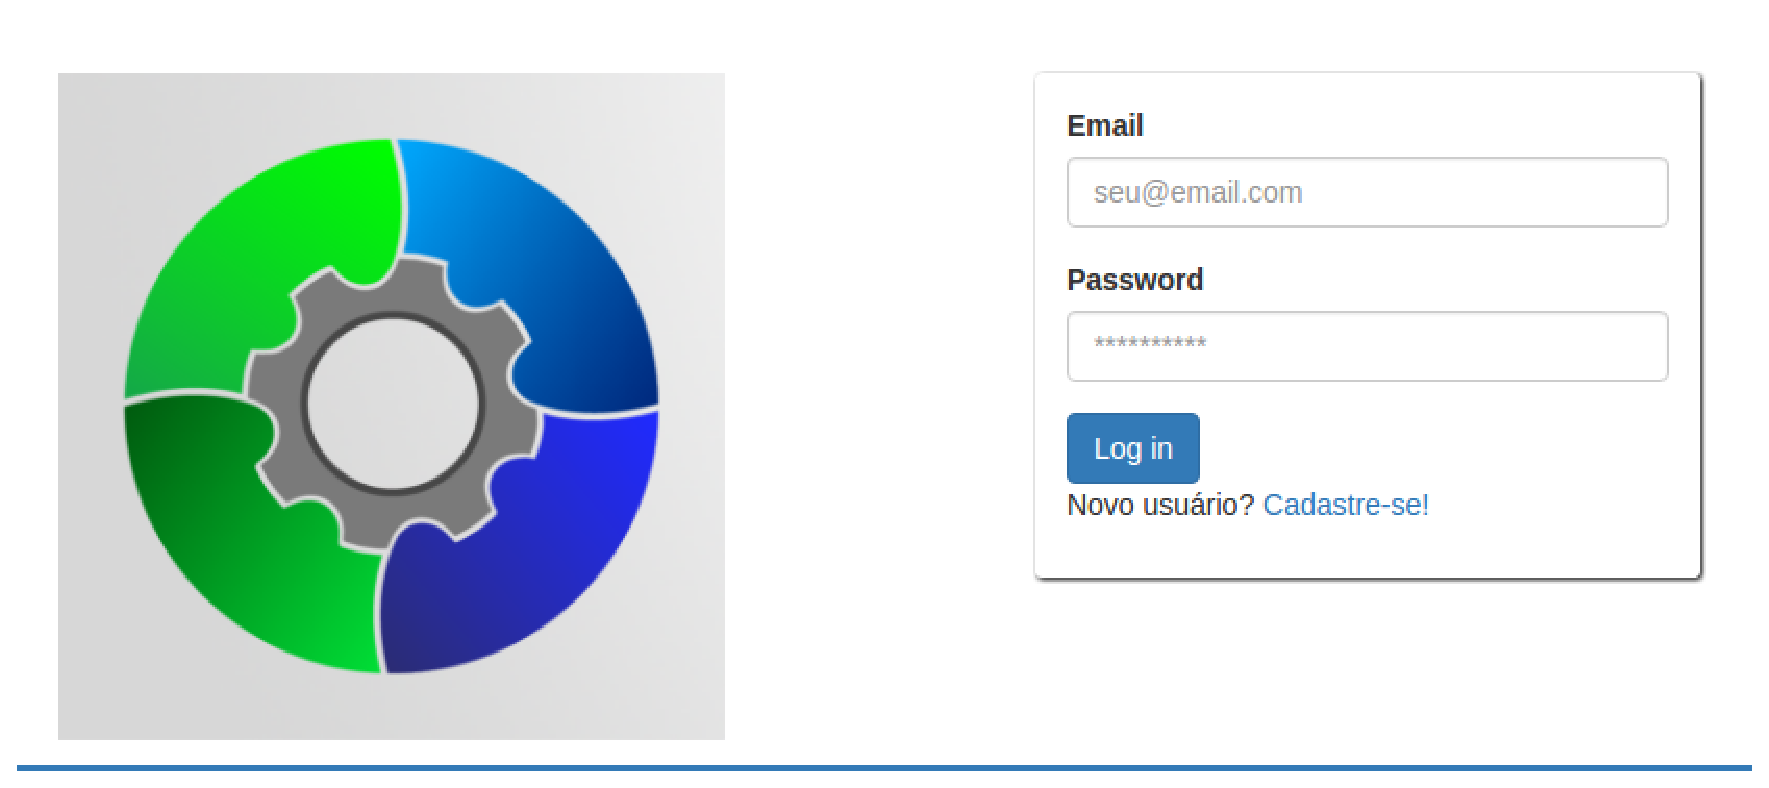
\includegraphics[keepaspectratio=true,scale=0.6]{figuras/user-login.eps}
  \caption{Tela de login}
\end{figure}


\begin{figure}[!ht]
  \centering
  \label{task_list}
    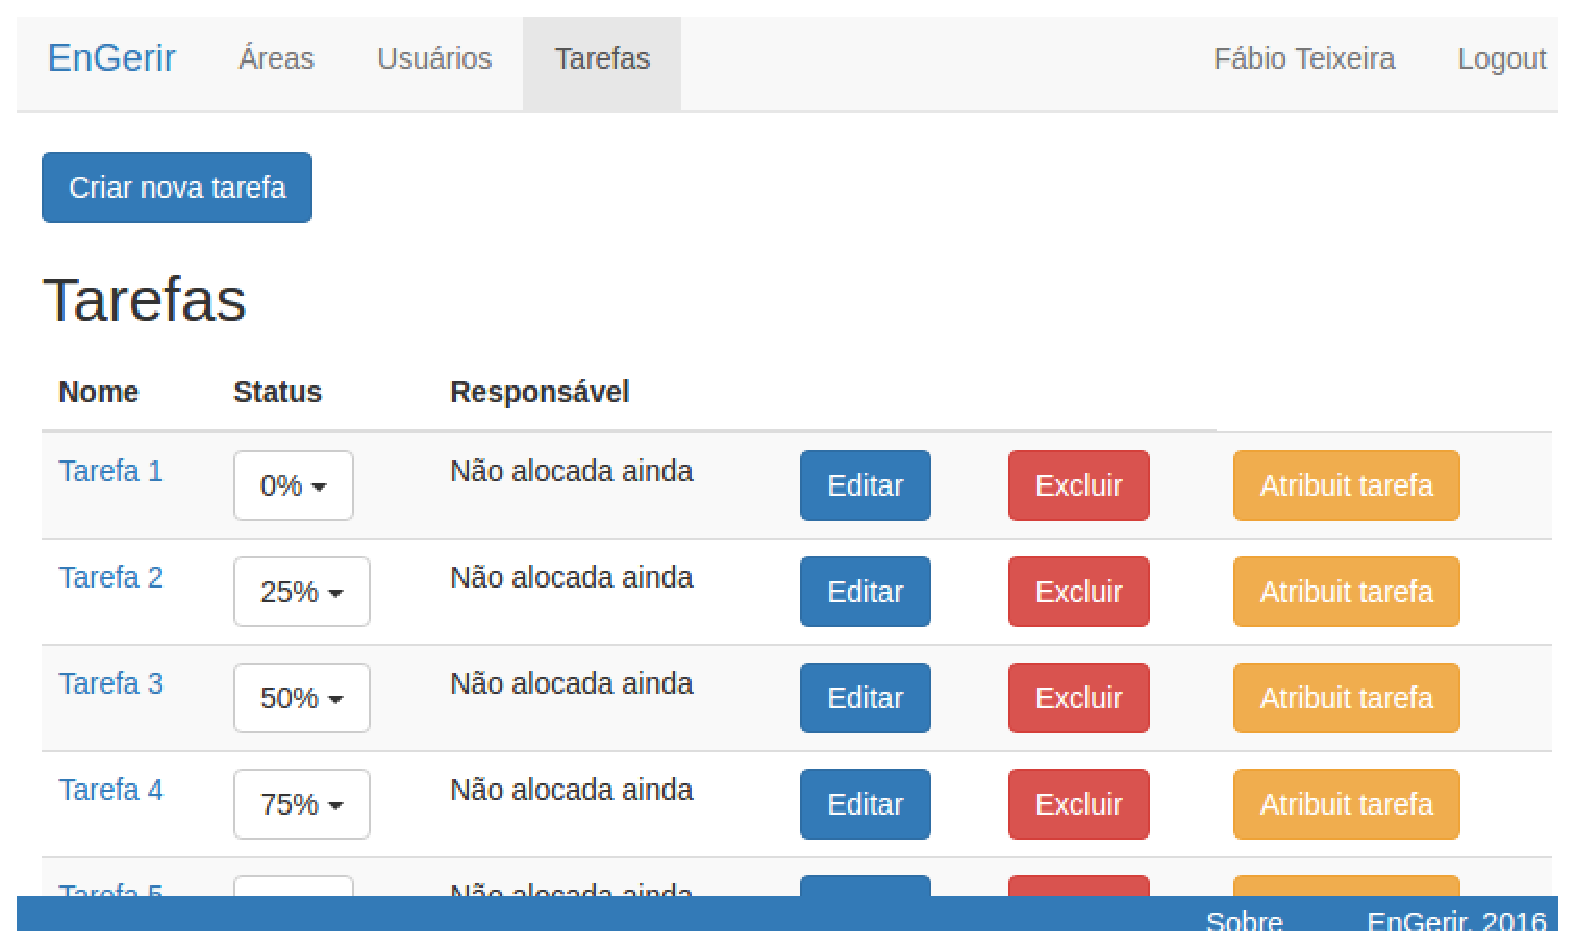
\includegraphics[keepaspectratio=true,scale=0.6]{figuras/task-list.eps}
  \caption{Lista de tarefas}
\end{figure}


\begin{figure}[!ht]
  \centering
  \label{user_edit}
    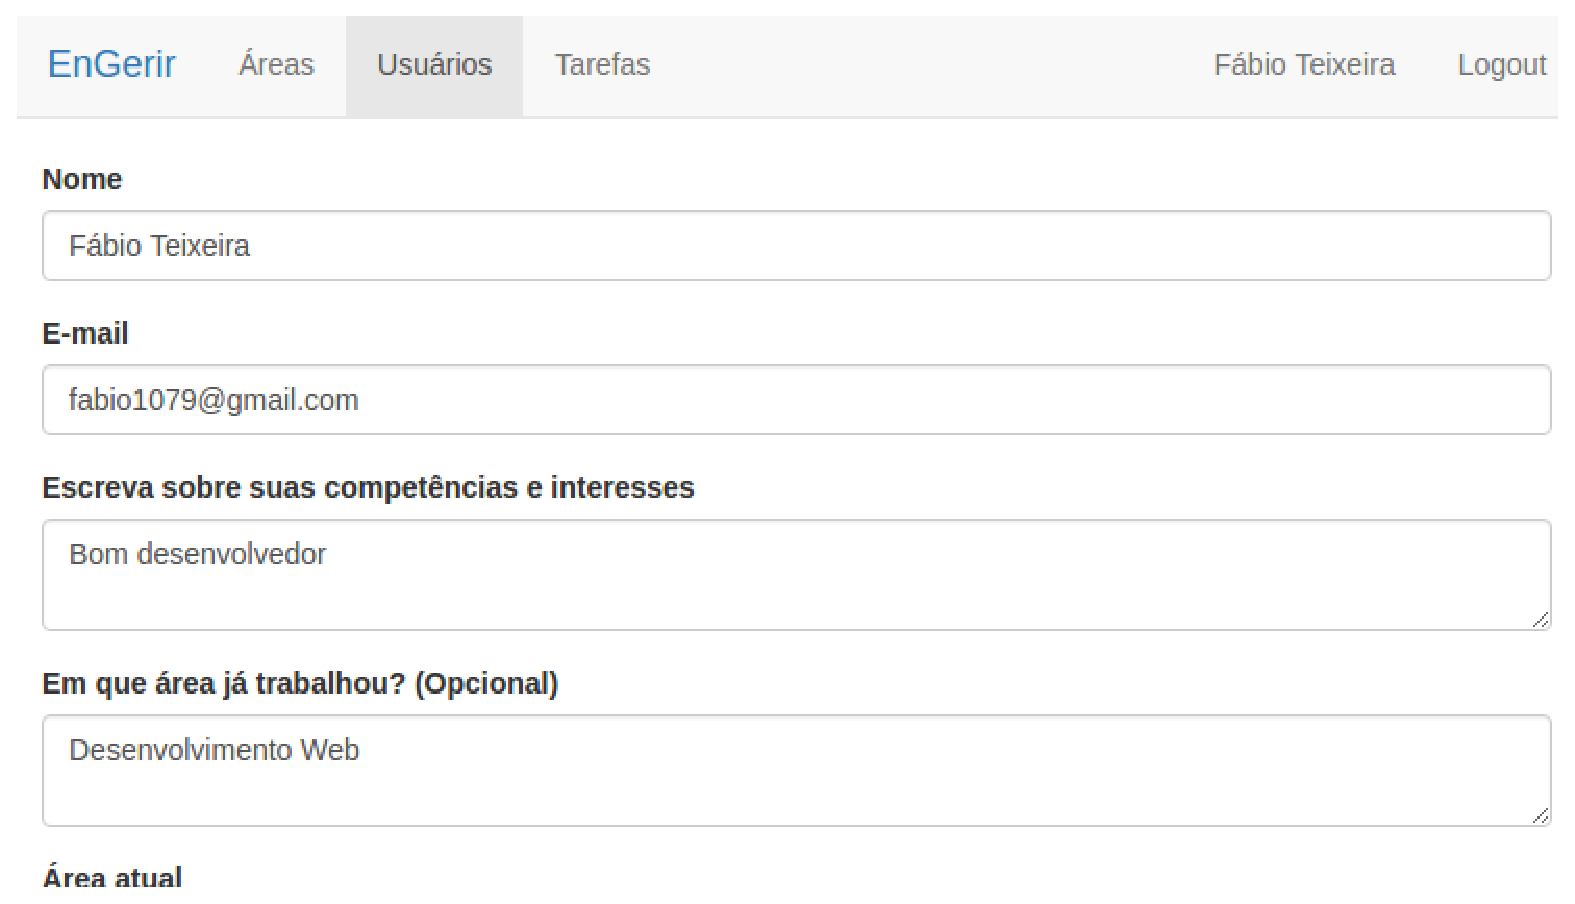
\includegraphics[keepaspectratio=true,scale=0.6]{figuras/user-edit.eps}
  \caption{Edição dos dados do usuário}
\end{figure}
